%%%%%%%%%%%%%%%%%%%%%%%%%%%%%%%%%%%%%%%%%%%%%%%%%
%%%%%%%%%%%%%%%%%%%%%%%%%%%%%%%%%%%%%%%%%%%%%%%%%
%%% Maxime Ulysse Garcia, max@ithake.eu, 2013 %%%
%%%                                           %%%
%%%    Questions and suggestions WELCOMED!    %%%
%%%                                           %%%
%%% This thesis template largely derives from %%%
%%%      Charles Chapple, Robert Castelo      %%%
%%%    Sergio Mendoza and Sergi Castellano    %%%
%%%       Under GNU/GPL copyleft license      %%%
%%%                                           %%%
%%%   FEEL FREE TO USE IT AND IMPROVE IT!!!   %%%
%%%                                           %%%
%%%%%%%%%%%%%%%%%%%%%%%%%%%%%%%%%%%%%%%%%%%%%%%%%
%%%%%%%%%%%%%%%%%%%%%%%%%%%%%%%%%%%%%%%%%%%%%%%%%

%%%%%%%%%%%%%%%%%%%%%%%%%%%%%%%%%%%%%%%%%%%%%%%%%
%%%%%%%%%%%%%%%%%%%%%%%%%%%%%%%%%%%%%%%%%%%%%%%%%
%%% Maxime Ulysse Garcia, max@ithake.eu, 2013 %%%
%%%                                           %%%
%%%    Questions and suggestions WELCOMED!    %%%
%%%                                           %%%
%%% This thesis template largely derives from %%%
%%%      Charles Chapple, Robert Castelo      %%%
%%%    Sergio Mendoza and Sergi Castellano    %%%
%%%       Under GNU/GPL copyleft license      %%%
%%%                                           %%%
%%%   FEEL FREE TO USE IT AND IMPROVE IT!!!   %%%
%%%                                           %%%
%%%%%%%%%%%%%%%%%%%%%%%%%%%%%%%%%%%%%%%%%%%%%%%%%
%%% Preamble: LaTeX parameters and extensions %%%
%%%%%%%%%%%%%%%%%%%%%%%%%%%%%%%%%%%%%%%%%%%%%%%%%

%%%%%%%%%%%%%%%%%%%%%%%%%%%%%%%%%%%%%%%%%%%%%%%%%
%%%               Document type               %%%
%%%%%%%%%%%%%%%%%%%%%%%%%%%%%%%%%%%%%%%%%%%%%%%%%
% While working to see output errors
%\documentclass[draft,pdftex,oneside]{book}

% To produce final printable version
\documentclass[pdftex,oneside]{book}

%%%%%%%%%%%%%%%%%%%%%%%%%%%%%%%%%%%%%%%%%%%%%%%%%
%%%              Tweaking errors              %%%
%%%%%%%%%%%%%%%%%%%%%%%%%%%%%%%%%%%%%%%%%%%%%%%%%

% To remove "No room for a new \dimen" when using tikz
\RequirePackage{etex}
% For fancyhdr
\setlength{\headheight}{13pt}

%%%%%%%%%%%%%%%%%%%%%%%%%%%%%%%%%%%%%%%%%%%%%%%%%
%%%             Our own style file            %%%
%%%%%%%%%%%%%%%%%%%%%%%%%%%%%%%%%%%%%%%%%%%%%%%%%

% Style file for this template myThesis.sty
\RequirePackage{myThesis}

%%%%%%%%%%%%%%%%%%%%%%%%%%%%%%%%%%%%%%%%%%%%%%%%%
%%%                   Colors                  %%%
%%%%%%%%%%%%%%%%%%%%%%%%%%%%%%%%%%%%%%%%%%%%%%%%%

\RequirePackage[usenames,
	dvipsnames,
	svgnames,
	table]{xcolor}

%%%%%%%%%%%%%%%%%%%%%%%%%%%%%%%%%%%%%%%%%%%%%%%%%
%%%                Paper layout               %%%
%%%%%%%%%%%%%%%%%%%%%%%%%%%%%%%%%%%%%%%%%%%%%%%%% 

\RequirePackage[paperwidth=170mm,
	paperheight=240mm,
	hmargin={2cm,1cm},
	vmargin={2cm,1.75cm},
	headheight=14pt]{geometry}

%%%%%%%%%%%%%%%%%%%%%%%%%%%%%%%%%%%%%%%%%%%%%%%%%
%%%                  Headings                 %%%
%%%%%%%%%%%%%%%%%%%%%%%%%%%%%%%%%%%%%%%%%%%%%%%%%

%For memoir class
\let\footruleskip\undefined

% To produce nice headings
\RequirePackage{fancyhdr}
\pagestyle{fancy}

% Big first letter.
\RequirePackage{lettrine}
\newcommand{\mylettrine}[1]{\lettrine[lines=3,lhang=.1]{#1}}

% Fancy looking boxes
\RequirePackage{tcolorbox}

%%%%%%%%%%%%%%%%%%%%%%%%%%%%%%%%%%%%%%%%%%%%%%%%%
%%%            Marks and draftmarks           %%%
%%%%%%%%%%%%%%%%%%%%%%%%%%%%%%%%%%%%%%%%%%%%%%%%%

\newcommand{\myversion}{V 0.7}

\renewcommand{\chaptermark}[1]{\markboth{\thechapter. #1}{}}
\renewcommand{\sectionmark}[1]{\markright{\thesection\ #1}}

\lfoot{}
\rfoot{}

% Normal marks
\lhead[\fancyplain{}{\sffamily\thepage}]{\fancyplain{}{\sffamily\rightmark}}
\rhead[\fancyplain{}{\sffamily\leftmark}]{\fancyplain{}{\sffamily\thepage}}
\cfoot{}

%Draftmarks
%\lhead[\fancyplain{}{\sffamily\thepage}]{\fancyplain{}{\sffamily\textcolor{blue}{DRAFT} \rightmark}}
%\rhead[\fancyplain{}{\sffamily\leftmark}]{\fancyplain{}{\sffamily\thepage}}
%\cfoot{\textcolor{blue}{\myversion}}

%%% Line Spacing %%%
\RequirePackage{setspace}

%%%%%%%%%%%%%%%%%%%%%%%%%%%%%%%%%%%%%%%%%%%%%%%%%
%%%                PDF commands               %%%
%%%%%%%%%%%%%%%%%%%%%%%%%%%%%%%%%%%%%%%%%%%%%%%%%

% To produce final version
\RequirePackage{pdfpages}

% Used in each \%includepdf call unless overwritten locally
\includepdfset{frame=false,pagecommand={\thispagestyle{fancy}}}

%%%%%%%%%%%%%%%%%%%%%%%%%%%%%%%%%%%%%%%%%%%%%%%%%
%%%                  Figures                  %%%
%%%%%%%%%%%%%%%%%%%%%%%%%%%%%%%%%%%%%%%%%%%%%%%%%

% Path to figures
\graphicspath{{figures//}}
% To include graphics
\RequirePackage{graphicx}
% To wrap text
\RequirePackage{wrapfig}
% to draw Figures
\RequirePackage{tikz}
% to rotate figures and tables
\RequirePackage{rotating}

%%%%%%%%%%%%%%%%%%%%%%%%%%%%%%%%%%%%%%%%%%%%%%%%%
%%%                 Equations                 %%%
%%%%%%%%%%%%%%%%%%%%%%%%%%%%%%%%%%%%%%%%%%%%%%%%%

\RequirePackage{mathtools}

% Redefine the square root:
\let\oldsqrt\sqrt
\def\sqrt{\mathpalette\DHLhksqrt}
\def\DHLhksqrt#1#2{
	\setbox0=\hbox{$#1\oldsqrt{#2\,}$}\dimen0=\ht0
	\advance\dimen0-0.2\ht0
	\setbox2=\hbox{\vrule height\ht0 depth -\dimen0}
	{\box0\lower0.4pt\box2}}

%%%%%%%%%%%%%%%%%%%%%%%%%%%%%%%%%%%%%%%%%%%%%%%%%
%%%                Big numbers                %%%
%%%%%%%%%%%%%%%%%%%%%%%%%%%%%%%%%%%%%%%%%%%%%%%%%

\RequirePackage{numprint}

%%%%%%%%%%%%%%%%%%%%%%%%%%%%%%%%%%%%%%%%%%%%%%%%%
%%%                   Lists                   %%%
%%%%%%%%%%%%%%%%%%%%%%%%%%%%%%%%%%%%%%%%%%%%%%%%%

% Provides a new environnement to do a list
\newenvironment{mylist}[1]{
	\begin{list}{}{
		\settowidth{\labelwidth}{#1:}
		\setlength{\labelsep}{0.5cm}
		\setlength{\leftmargin}{\labelwidth}
		\addtolength{\leftmargin}{\labelsep}
		\setlength{\rightmargin}{0pt}
		\setlength{\parsep}{0.5ex plus 0.2ex minus 0.1ex}
		\setlength{\itemsep}{0 ex plus 0.2ex}
		\renewcommand{\makelabel}[1]{\textbf{##1}\hfil}
		}
	}
{\end{list}}

%%%%%%%%%%%%%%%%%%%%%%%%%%%%%%%%%%%%%%%%%%%%%%%%%
%%%                  Acronyms                 %%%
%%%%%%%%%%%%%%%%%%%%%%%%%%%%%%%%%%%%%%%%%%%%%%%%%

\RequirePackage{suffix}
\RequirePackage[printonlyused]{acronym}

%%%%%%%%%%%%%%%%%%%%%%%%%%%%%%%%%%%%%%%%%%%%%%%%%
%%%                  Verbatim                 %%%
%%%%%%%%%%%%%%%%%%%%%%%%%%%%%%%%%%%%%%%%%%%%%%%%%

\RequirePackage{moreverb}

%%%%%%%%%%%%%%%%%%%%%%%%%%%%%%%%%%%%%%%%%%%%%%%%%
%%%                 References                %%%
%%%%%%%%%%%%%%%%%%%%%%%%%%%%%%%%%%%%%%%%%%%%%%%%%

\RequirePackage[round,comma,numbers,super,sort&compress]{natbib}

%%%%%%%%%%%%%%%%%%%%%%%%%%%%%%%%%%%%%%%%%%%%%%%%%
%%%                   Index                   %%%
%%%%%%%%%%%%%%%%%%%%%%%%%%%%%%%%%%%%%%%%%%%%%%%%%

\RequirePackage{makeidx}
\makeindex

%%%%%%%%%%%%%%%%%%%%%%%%%%%%%%%%%%%%%%%%%%%%%%%%%
%%%                   Fonts                   %%%
%%%%%%%%%%%%%%%%%%%%%%%%%%%%%%%%%%%%%%%%%%%%%%%%%

\RequirePackage{palatino}
\RequirePackage{amsfonts}

%%%%%%%%%%%%%%%%%%%%%%%%%%%%%%%%%%%%%%%%%%%%%%%%%
%%%               URL inclusion               %%%
%%%%%%%%%%%%%%%%%%%%%%%%%%%%%%%%%%%%%%%%%%%%%%%%%

\RequirePackage[pdftex,
	colorlinks=true,
	linkcolor=black,
	menucolor=red,
	pdfhighlight=/P,
	citecolor=MidnightBlue,
	urlcolor=BrickRed,
	linktocpage=false]{hyperref}
%Enter URLs like this: \url{http://ithake.eu/}

%%%%%%%%%%%%%%%%%%%%%%%%%%%%%%%%%%%%%%%%%%%%%%%%%
%%%               Defining terms              %%%
%%%%%%%%%%%%%%%%%%%%%%%%%%%%%%%%%%%%%%%%%%%%%%%%%

\def\myauthor{Firstname Lastname}

\def\mytitlefr{Titre en français}

\def\mytitleen{English title}

\def\myabstractfr{\blindtext}

\def\myabstracten{\blindtext}

\def\mykeywordsfr{mots-clés; français}

\def\mykeywordsen{English; Keywords}

% To get subscript easily
\newcommand{\textunderscript}[1]{$_{\text{#1}}$}

% To get e and er in superscript easily
\newcommand{\eme}{\textsuperscript{e} }
\newcommand{\er}{\textsuperscript{er} }

% To get CO2 and O2 easily
\newcommand{\COO}{CO\textunderscript{2} }
\newcommand{\OO}{O\textunderscript{2} }

% shorther command for boldface
\newcommand{\bb}[1]{\textbf{#1}}

%%% to add an empty page, output pending figures and resume in an odd-numbered one %%%

\newcommand{\clearemptypage}{\newpage\thispagestyle{empty}\mbox{}}

\newcommand{\clearemptydoublepage}{
	\clearemptypage
	\if@twoside
		\ifodd
			\clearemptypage
		\fi
	\fi}

%%%%%%%%%%%%%%%%%%%%%%%%%%%%%%%%%%%%%%%%%%%%%%%%%
%%%                 PDF infos                 %%%
%%%%%%%%%%%%%%%%%%%%%%%%%%%%%%%%%%%%%%%%%%%%%%%%%

\hypersetup{
	pdftitle		= {\mytitlefr},
	pdfsubject		= {subject},
	pdfkeywords		= {\mykeywordsfr},
	pdfauthor		= {\myauthor},
	pdfcreator		= {\LaTeX},
	pdfproducer		= {pdfeTeX-0.\the\pdftexversion\pdftexrevision}
	pdfpagemode		= FullScreen,
	pdffitwindow	= true}

\AtBeginDocument{\pdfpagewidth=176mm\pdfpageheight=250mm}

%%%%%%%%%%%%%%%%%%%%%%%%%%%%%%%%%%%%%%%%%%%%%%%%%
%%%                 Paragraphs                %%%
%%%%%%%%%%%%%%%%%%%%%%%%%%%%%%%%%%%%%%%%%%%%%%%%%

\setlength{\parskip}{1ex plus0.2ex minus0.2ex}

%%%%%%%%%%%%%%%%%%%%%%%%%%%%%%%%%%%%%%%%%%%%%%%%%
%%%                 Footnotes                 %%%
%%%%%%%%%%%%%%%%%%%%%%%%%%%%%%%%%%%%%%%%%%%%%%%%%

% Vertical spacing between footnotes
\setlength{\footnotesep}{2ex}

% Rule height, width and space
\renewcommand{\footnoterule}{\noindent\rule{5cm}{.1ex}\vspace{1.5ex}}

% That's all folks!
 % Call layout and other LaTeX parameters

%%%%%%%%%%%%%%%%%%%%%%%%%%%%%%%%%%%%%%%%%%%%%%%%%
%%%   Body: text with some control commands   %%%
%%%%%%%%%%%%%%%%%%%%%%%%%%%%%%%%%%%%%%%%%%%%%%%%%

%%%%%%%%%%%%%%%%%%%%%%%%%%%%%%%%%%%%%%%%%%%%%%%%%
%%%       The whole writing starts here       %%%
%%%         divided into frontmatter,         %%%
%%%         mainmatter and backmatter         %%%
%%%%%%%%%%%%%%%%%%%%%%%%%%%%%%%%%%%%%%%%%%%%%%%%%

% Each \input command searches for a .tex file in a directory

% Build the minitoc
\dominitoc
\nomtcrule

% Set how many levels of subsections are listed in the Table Of Contents (TOC)
\setcounter{secnumdepth}{5}
\setcounter{tocdepth}{5}

% The main body lies within the \begin{document} and \end{document} commands.
\begin{document}

%%%%%%%%%%%%%%%%%%%%%%%%%%%%%%%%%%%%%%%%%%%%%%%%%
%%%                frontmatter                %%%
%%%%%%%%%%%%%%%%%%%%%%%%%%%%%%%%%%%%%%%%%%%%%%%%%

\frontmatter
	\addcontentsline{toc}{chapter}{Thèse}
	\thispagestyle{empty}
	\begin{center}
		\avantgarLarge University\\[1ex]
		\avantgar Faculty\\[1ex]
		\avantgar Doctoral School\\[3ex]
	\end{center}

	\begin{center}
		\avantgarboldHuge THÈSE\\[1.5ex]

		\avantgarlarge First version\\[1ex]
		\avantgarlarge \today\\[1ex]
		\avantgarLarge \myauthor\\[1ex]

		\avantgarboldHuge \mytitlefr\\[2ex]

		\avantgarlarge Speciality\\[5ex]

		\avantgarlarge Jury :\\[1ex]
		\begin{tabular}{llll}
			{\Large M.} & {\Large\textsc{Una}}			& {\large Labo}	& {\large(Role)}	\\
			{\Large M.} & {\Large\textsc{Secunda}}		& {\large Labo}	& {\large(Role)}	\\
			{\Large M.} & {\Large\textsc{Teriari}}		& {\large Labo}	& {\large(Role)}	\\
			{\Large M.} & {\Large\textsc{Quaternary}} 	& {\large Labo}	& {\large(Role)}	\\
		\end{tabular}
	\end{center}

	\clearemptypage

	\thispagestyle{empty}
% Laboratory and intitutions
\noindent\textsf{\blindtext}
\vspace{.7cm}

% Logos
\begin{center}
	\avantgarLarge LOGO1\\[1ex]
	\avantgarLarge LOGO2\\[1ex]
	\avantgarLarge LOGO3
\end{center}

% Funding
\vspace{.7cm}
\noindent\textsf{\blindtext}
				% Institutional logos
	\clearemptypage

	\thispagestyle{empty}

\vspace*{5cm}
% Dedicatory
\begin{flushright}
	\sffamily
		To whoever you want
\end{flushright}
			% Dedicatory
	\chapter*{Remerciements}

% Supervisors
\noindent{}\blindtext
\vspace{.5cm}

% Team + Laboratory
\noindent{}\blindtext
\vspace{.5cm}

% Friends
% Family
% Special someone	% Acknowledgements

%%%%%%%%%%%%%%%%%%%%%%%%%%%%%%%%%%%%%%%%%%%%%%%%%
%%%             TOC, TOT, and TOF             %%%
%%%%%%%%%%%%%%%%%%%%%%%%%%%%%%%%%%%%%%%%%%%%%%%%%

	% For a more compact layout 
	\setlength{\parskip}{0.4ex plus0.2ex minus0.2ex}

	% Main TOC
	\tableofcontents
	\mtcaddchapter	% prevent shifting

	% TOT
	\listoftables
	\mtcaddchapter	% prevent shifting

	% TOF
	\listoffigures
	\mtcaddchapter	% prevent shifting
	\mtcaddchapter	% prevent shifting

%%%%%%%%%%%%%%%%%%%%%%%%%%%%%%%%%%%%%%%%%%%%%%%%%
%%%                 mainmatter                %%%
%%%%%%%%%%%%%%%%%%%%%%%%%%%%%%%%%%%%%%%%%%%%%%%%%

\mainmatter
	\clearemptydoublepage

	\singlespacing

\mychapter{red!45!black}{Introduction}
	\sectionred*{Résumé}
		\begin{center}
				\begin{tcolorbox}[colback=red!5!white,colframe=red!45!black,arc=0mm]

					\sffamily
						\blindtext
					\end{tcolorbox}
					\vspace{5ex}
					\mtcsetdepth{minitoc}{1}
					\minitoc
		\end{center}
		\newpage

	\doublespacing

	\section{\textcolor{red!45!black}{First Part}}\label{sec:first1}
		\mylettrine{T}{}\blindtext

	\section{\textcolor{red!45!black}{Second Part}}\label{sec:second1}
		\mylettrine{T}{}\blindtext

		\subsection{\textcolor{red!45!black}{Sub-part 1}}\label{sub:part11}
					\mylettrine{T}{}\blindtext

		\subsection{\textcolor{red!45!black}{Sub-part 2}}\label{sub:part21}
					\mylettrine{T}{}\blindtext


	\section{\textcolor{red!45!black}{Conclusion}}

		\mylettrine{T}{}\blindtext
			% State of the art
	\clearemptydoublepage

	\singlespacing

\mychapter{green!45!black}{Methods}
	\sectiongreen*{Résumé}
		\begin{center}
				\begin{tcolorbox}[colback=green!5!white,colframe=green!45!black,arc=0mm]

					\sffamily
						\blindtext
					\end{tcolorbox}
					\vspace{5ex}
					\mtcsetdepth{minitoc}{1}
					\minitoc
		\end{center}
		\newpage

	\doublespacing

	\section{\textcolor{green!45!black}{First Part}}\label{sec:first2}
		\mylettrine{T}{}\blindtext

	\section{\textcolor{green!45!black}{Second Part}}\label{sec:second2}
		\mylettrine{T}{}\blindtext

		\subsection{\textcolor{green!45!black}{Sub-part 1}}\label{sub:part12}
					\mylettrine{T}{}\blindtext

		\subsection{\textcolor{green!45!black}{Sub-part 2}}\label{sub:part22}
					\mylettrine{T}{}\blindtext


	\section{\textcolor{green!45!black}{Conclusion}}

		\mylettrine{T}{}\blindtext
				% Material & Methods + Supplementary Information
	\clearemptydoublepage

	\singlespacing

\mychapter{green!45!black}{Results}
	\sectiongreen*{Résumé}
		\begin{center}
				\begin{tcolorbox}[colback=green!5!white,colframe=green!45!black,arc=0mm]

					\sffamily
						\blindtext
					\end{tcolorbox}
					\vspace{5ex}
					\mtcsetdepth{minitoc}{1}
					\minitoc
		\end{center}
		\newpage

	\doublespacing

	\section{\textcolor{green!45!black}{First Part}}\label{sec:first3}
		\mylettrine{T}{}\citep{key001}\blindtext

	\section{\textcolor{green!45!black}{Second Part}}\label{sec:second3}
		\mylettrine{T}{}\blindtext

		\subsection{\textcolor{green!45!black}{Sub-part 1}}\label{sub:part13}
					\mylettrine{T}{}\blindtext

		\subsection{\textcolor{green!45!black}{Sub-part 2}}\label{sub:part23}
					\mylettrine{T}{}\blindtext


	\section{\textcolor{green!45!black}{Conclusion}}

		\mylettrine{T}{}\blindtext
				% Got papers? great!
	\clearemptydoublepage

	\singlespacing

\mychapter{green!45!black}{Results2}
	\sectiongreen*{Résumé}
		\begin{center}
				\begin{tcolorbox}[colback=green!5!white,colframe=green!45!black,arc=0mm]

					\sffamily
						\blindtext
					\end{tcolorbox}
					\vspace{5ex}
					\mtcsetdepth{minitoc}{1}
					\minitoc
		\end{center}
		\newpage

	\doublespacing

	\section{\textcolor{green!45!black}{First Part}}\label{sec:first3}
		\mylettrine{T}{}\citep{key002}\blindtext

	\section{\textcolor{green!45!black}{Second Part}}\label{sec:second3}
		\mylettrine{T}{}\blindtext

		\subsection{\textcolor{green!45!black}{Sub-part 1}}\label{sub:part13}
					\mylettrine{T}{}\blindtext

		\subsection{\textcolor{green!45!black}{Sub-part 2}}\label{sub:part23}
					\mylettrine{T}{}\blindtext


	\section{\textcolor{green!45!black}{Conclusion}}

		\mylettrine{T}{}\blindtext
				% Got more papers? wonderful!
	\clearemptydoublepage

	\singlespacing

\mychapter{blue!45!black}{Discussion}
	\sectionblue*{Résumé}
		\begin{center}
				\begin{tcolorbox}[colback=blue!5!white,colframe=blue!45!black,arc=0mm]

					\sffamily
						\blindtext
					\end{tcolorbox}
					\vspace{5ex}
					\mtcsetdepth{minitoc}{1}
					\minitoc
		\end{center}
		\newpage

	\doublespacing

	\section{\textcolor{blue!45!black}{First Part}}\label{sec:first5}
		\mylettrine{T}{}\blindtext

	\section{\textcolor{blue!45!black}{Second Part}}\label{sec:second5}
		\mylettrine{T}{}\blindtext

		\subsection{\textcolor{blue!45!black}{Sub-part 1}}\label{sub:part15}
					\mylettrine{T}{}\blindtext

		\subsection{\textcolor{blue!45!black}{Sub-part 2}}\label{sub:part25}
					\mylettrine{T}{}\blindtext


	\section{\textcolor{blue!45!black}{Conclusion}}

		\mylettrine{T}{}\blindtext
			% Make sense of the whole of it
	\clearemptydoublepage

	\singlespacing

\mychapter{blue!45!black}{Conclusion}
	\newpage

\doublespacing

	\section*{\textcolor{blue!45!black}{Conclusion}}
		\mylettrine{T}{}\blindtext
		\Blindtext
			% Your contribution in short points
	\clearemptydoublepage

	\begin{appendices}					% Appendices
		\singlespacing

\mynochapter{white!15!black}{Annexes}\addstarredchapter{Annexes}
	\sectiongrey*{Détail}
		\begin{center}
			\begin{tcolorbox}[colback=black!5!white,colframe=white!15!black,arc=0mm]
				\sffamily
				\blindtext
			\end{tcolorbox}
			\vspace{5ex}
			\mtcsetdepth{minitoc}{1}
			\minitoc
		\end{center}
		% Explaining what is in your appendices
		\mychapter{white!15!black}{Publications}
		\section{\textcolor{white!15!black}{\emph{Best article ever}}}\label{app:article1}
			\citep{key001}
			\blindtext
			\blindtext
			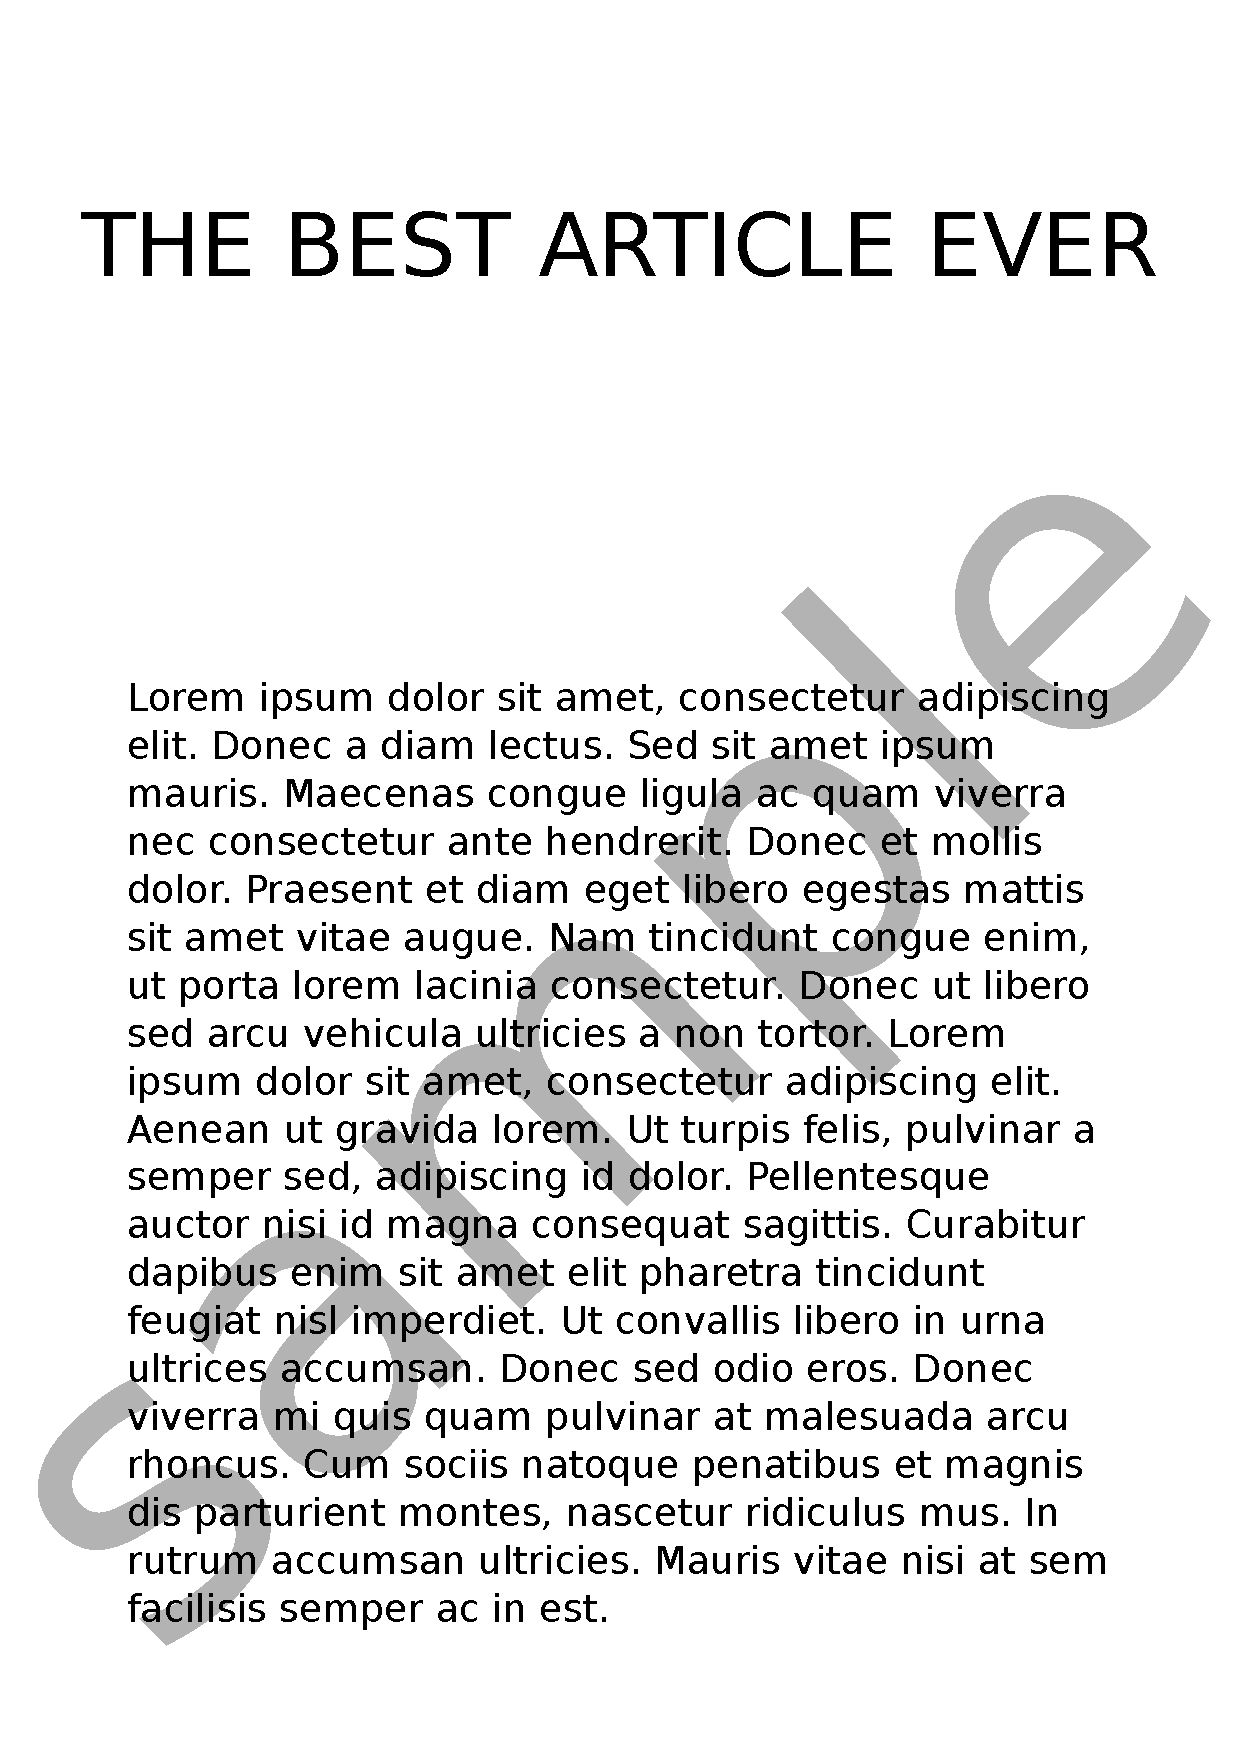
\includepdf[pages={1}, offset=5mm 0mm]{articles/sample.pdf}

		\section{\textcolor{white!15!black}{\emph{Second best article ever}}}\label{app:article2}
			\citep{key002}
			\blindtext
			\blindtext
			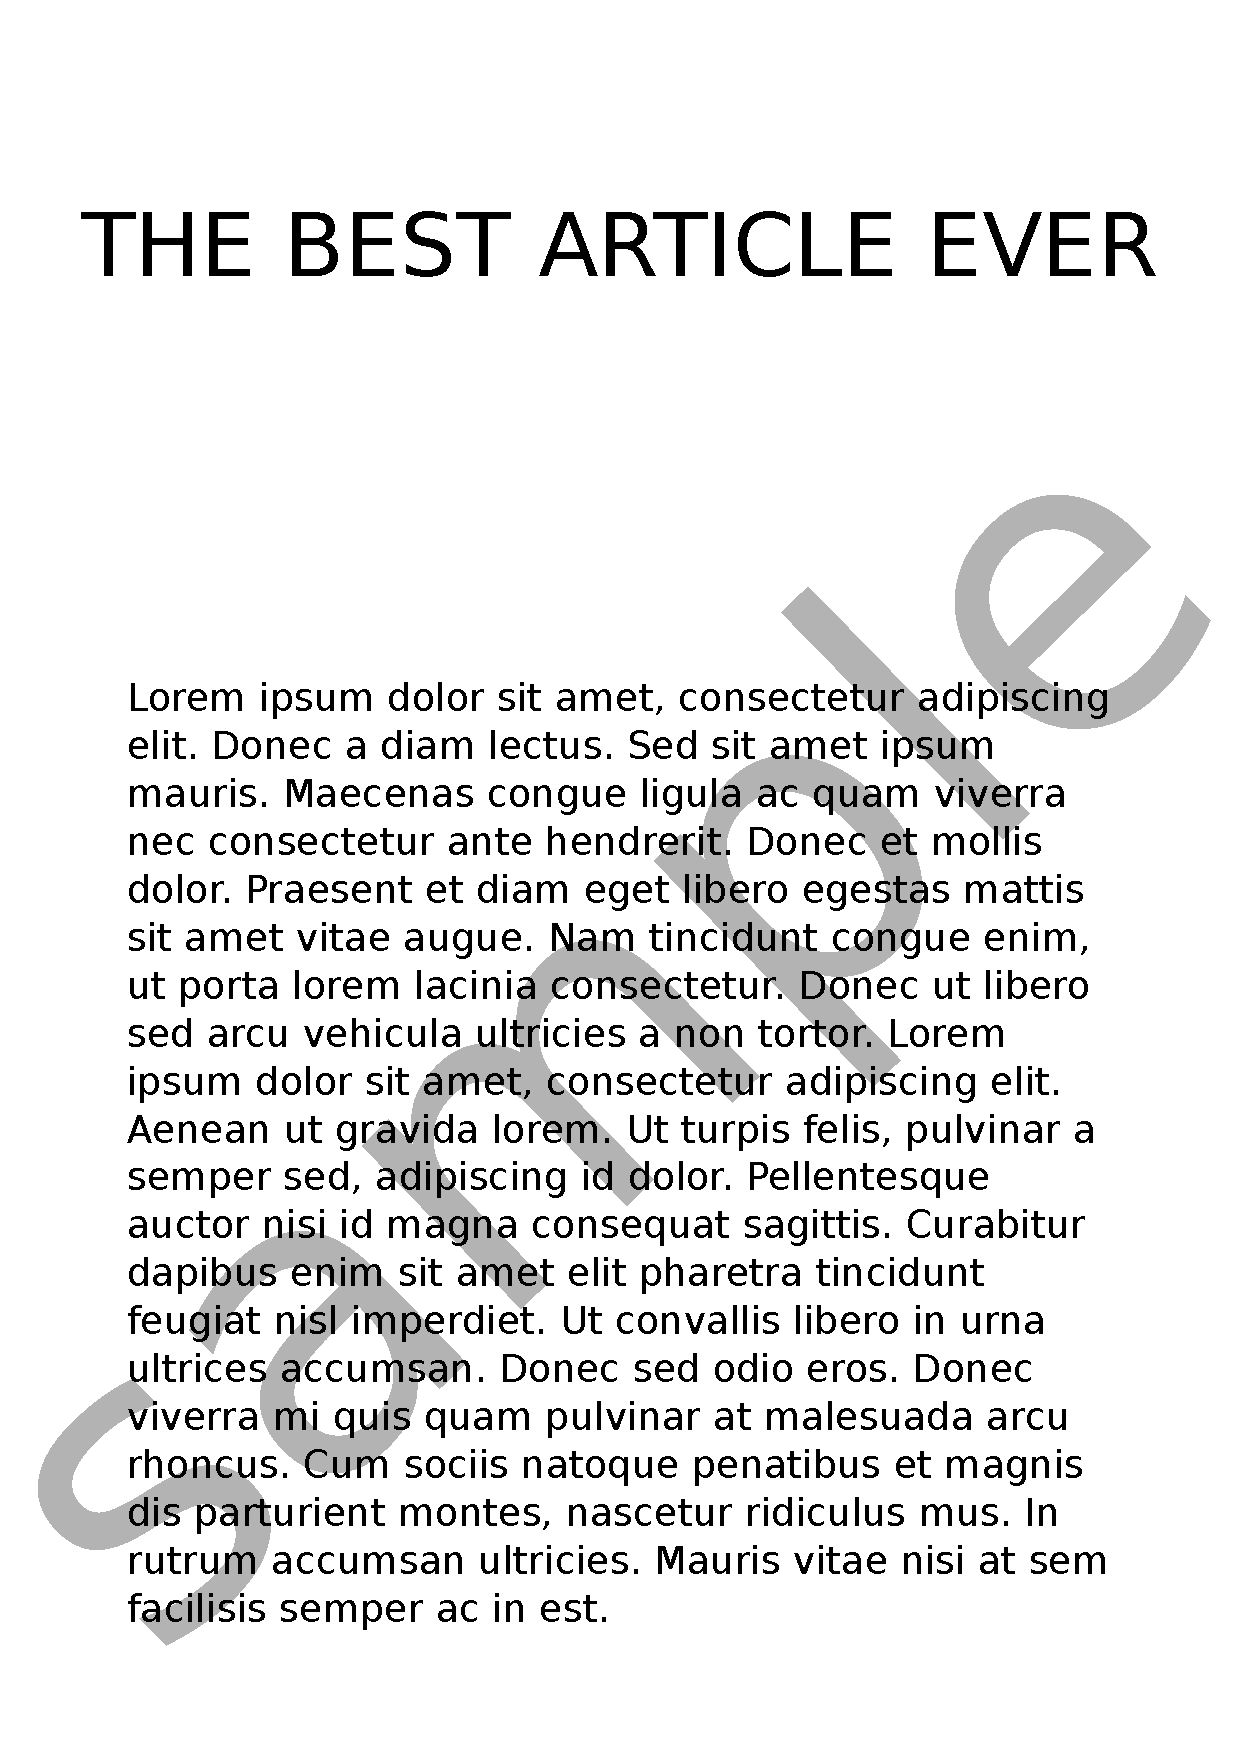
\includepdf[pages={1}, offset=5mm 0mm]{articles/sample.pdf}
	% All your publications
	\end{appendices}

%%%%%%%%%%%%%%%%%%%%%%%%%%%%%%%%%%%%%%%%%%%%%%%%%
%%%                 backmatter                %%%
%%%%%%%%%%%%%%%%%%%%%%%%%%%%%%%%%%%%%%%%%%%%%%%%%

\backmatter
	\singlespacing
	\bibliography{bibliography/biblio}	% Your bibliography
	\bibliographystyle{unsrtnat}		% The bibliography style
	\clearemptydoublepage

	\singlespacing

\mynochapter{white!15!black}{Colophon}
\addstarredchapter{Colophon}
	\begin{center}
		\begin{tcolorbox}[colback=black!5!white,colframe=white!15!black,arc=0mm]
			\sffamily
			Ce document a été préparé à l'aide du logiciel de composition typographique {\LaTeX} et de l'éditeur de texte Sublime Text 3. Il a été compilé via pdfTeX 3.1415926-1.40.10 (TeX Live 2009/Debian) sur un système GNU/Linux Ubuntu 13.04. Le template utilisé pour formater cette thèse est basé sur un template originel de Robert Castelo distribué sous licence GNU/GPL copyleft. La version actuelle de ce template est disponible sur \url{http://github.com/MaxUlysse/myThesis/}.\\
			This document was prepared with {\LaTeX} and Sublime Text 3. It was compile via pdfTeX 3.1415926-1.40.10 (TeX Live 2009/Debian) on a GNU/Linux Ubuntu 13.04 system.
			The template used for this thesis is based on a original template by Robert Castelo shared under GNU/GPL copyleft license. The actual version is available on \url{http://github.com/MaxUlysse/myThesis/}.
		\end{tcolorbox}
	\end{center}
				% Small colophon to explain how it was made
	\clearemptydoublepage

	\phantomsection
	\addcontentsline{toc}{chapter}{Abstract}	
	{\small
	\begin{description}
		\item [Titre]		\hfill \\
			\mytitlefr
		\item [Résumé]		\hfill \\
			\myabstractfr
		\item [Mots-clés]	\hfill \\
			\mykeywordsfr
	\end{description}

	\begin{description}
		\item [Title]		\hfill \\
			\mytitleen
		\item [Abstract]	\hfill \\
			\myabstracten
		\item [Keywords]	\hfill \\
			\mykeywordsen
	\end{description}
}
				% Abstracts of your thesis

\end{document}

%%%%%%%%%%%%%%%%%%%%%%%%%%%%%%%%%%%%%%%%%%%%%%%%%
%       It's finally over, you made it !!!      %
%           Look for a postdoc now!!!           %
%                  Or a life...                 %
%%%%%%%%%%%%%%%%%%%%%%%%%%%%%%%%%%%%%%%%%%%%%%%%%